\documentclass[border=10pt]{standalone}
\usepackage{tikz}

\begin{document}

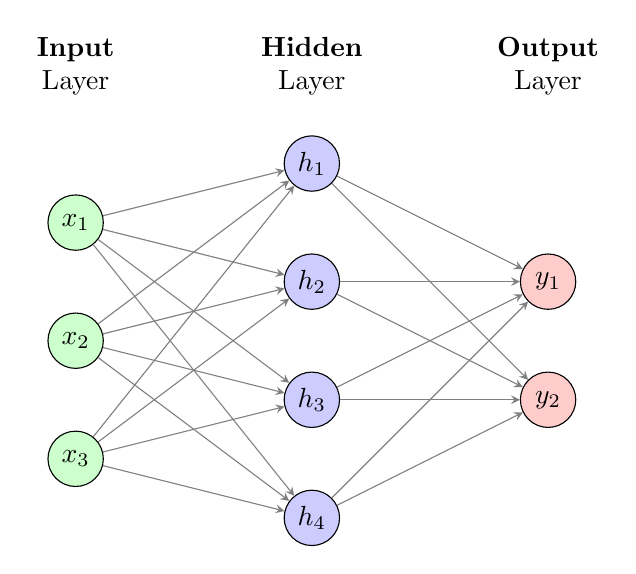
\begin{tikzpicture}[
    node distance=1.5cm and 2.5cm,
    neuron/.style={circle, draw=black, fill=blue!20, minimum size=20pt, inner sep=0pt},
    input neuron/.style={neuron, fill=green!20},
    output neuron/.style={neuron, fill=red!20},
    hidden neuron/.style={neuron, fill=blue!20},
    >=stealth
]

% Input layer
\foreach \i in {1,...,3} {
    \node[input neuron] (I-\i) at (0, -\i*1.5) {$x_{\i}$};
}

% Hidden layer
\foreach \j in {1,...,4} {
    \node[hidden neuron] (H-\j) at (3, -\j*1.5 + 0.75) {$h_{\j}$};
}

% Output layer
\foreach \k in {1,...,2} {
    \node[output neuron] (O-\k) at (6, -\k*1.5 - 0.75) {$y_{\k}$};
}

% Connections: Input -> Hidden
\foreach \i in {1,...,3} {
    \foreach \j in {1,...,4} {
        \draw[->, gray] (I-\i) -- (H-\j);
    }
}

% Connections: Hidden -> Output
\foreach \j in {1,...,4} {
    \foreach \k in {1,...,2} {
        \draw[->, gray] (H-\j) -- (O-\k);
    }
}

% Layer labels
\node[align=center, above] at (0, 0) {\textbf{Input}\\Layer};
\node[align=center, above] at (3, 0) {\textbf{Hidden}\\Layer};
\node[align=center, above] at (6, 0) {\textbf{Output}\\Layer};

\end{tikzpicture}

\end{document}
